\documentclass{beamer}
\graphicspath{{../graphics/}}
\usepackage{listings}
\usepackage{ulem}
\usepackage{subcaption}
\captionsetup{compatibility=false}
\usepackage[linesnumbered]{algorithm2e}
\usepackage{multicol}

\newcommand{\linespace}{\vspace{1em}}

\mode<presentation>
{
  \usetheme{Darmstadt}
  \setbeamertemplate{footline}[frame number]
  \setbeamertemplate{navigation symbols}{}
  \setbeamercovered{transparent}
}

\AtBeginSection[]
{
   \begin{frame}
        \frametitle{Content}
        \tableofcontents[sectionstyle=show/hide,subsectionstyle=show/show/hide]
   \end{frame}
}

\usepackage[danish]{babel}
\usepackage[T1]{fontenc}

\usepackage[utf8]{inputenc}

\usepackage{times}

\usepackage{tikz}
\usepackage{multirow}

\title[OHPAC]{Online Hotspot-based Predictions\\
for Aalborg City Bike}

\subtitle{SW701E14}

\author[SW701E14]{
Mikael Elkiær Christensen \\\and
Alexander Drægert \\\and
Mikkel Sandø Larsen \\\and
Stefan Marstrand Getreuer Micheelsen \\\and
Bruno Thalmann
}

\institute[Aalborg University]
{
  Software\\
  Aalborg University}

\date[CFP 2003]{January 28, 2015}

\begin{document}

% % % % % % % %
% INTRODUCTION
% % % % % % % %

\begin{frame}
  \titlepage
\end{frame}

\begin{frame}
    \frametitle{Content}
    \tableofcontents[sectionstyle=show/show,subsectionstyle=hide/hide/hide]
\end{frame}

% % % % %
% SLIDES
% % % % %

To counter the increasing energy and environmental issues, Aalborg Kommune implemented the CIVITAS-ARCHIMEDES project\cite{aalborgbycyklenbagcyklen}. As part of this project, city bikes were made publicly available for everyday use.
In order to maximize the number of users, the usage was cheap and easy but the bikes were well equipped and was of good quality\cite{cykelplanlaegning}.
To use a bike all you need to do is to place a 20DKK coin into a bike lock. When your ride is over and you lock the bike at the station, you will get your 20DKK back.
\section{Analysis}

\subsection{Aalborg City Bike}

% % % % % %
% Aalborg City Bike as basis
% % % % % %
\begin{frame}
\frametitle{Aalborg City Bike as basis}
\begin{columns}
\begin{column}{.45\textwidth}
\begin{block}{From aalborgbycyklen.dk:}
Take a citybike,
\begin{itemize}
\item when you parked your car and feel like riding along the promenade or harbour.
\item when it's Monday morning and your own bike has a flat tire.
\item when you want to swing by your friends house.
\end{itemize}
\end{block}
\end{column}
\begin{column}{.45\textwidth}
\begin{figure}
\includegraphics[width=\textwidth]{graphics/acb_bike}
\caption{An Aalborg City Bike (aalborgbycyklen.dk)}
\end{figure}
\end{column}
\end{columns}
\end{frame}

% % % % % %
% Aalborg City Bike facts
% % % % % %
\begin{frame}
\frametitle{Aalborg City Bike facts}
\begin{columns}
\begin{column}{.44\textwidth}
\begin{itemize}
\item 200 bikes
\begin{itemize}
\item 140 active
\end{itemize}
\item 21 bike stations
\begin{itemize}
\item Room for 170 bikes
\end{itemize}
\item Each bike has a lock, attached to a station
\item Unlock with 20 DKK coin, re-locking returns the coin
\end{itemize}
\end{column}
\begin{column}{.44\textwidth}
\begin{figure}
\includegraphics[width=\textwidth]{graphics/acb_gmaps}
\caption{Map of all bike stations in Aalborg/Nørresundby Area (aalborgbycyklen.dk)}
\end{figure}
\end{column}
\end{columns}
\end{frame}

% % % % % %
% Interview and existing systems
% % % % % %
\begin{frame}
\frametitle{Interview and existing systems}
{\Huge ?}
\end{frame}

% % % % % %
% Analysis summary
% % % % % %
\begin{frame}
\frametitle{Analysis summary}
\begin{columns}
\begin{column}{.45\textwidth}
\begin{block}{Problems\footnotemark}
\begin{enumerate}
\item Bikes left outside stations
\item Too few stations
\item Making short stops
\item No bikes at station
\item No way of knowing when a bike will arrive
\item Broken bikes
\end{enumerate}
\end{block}
\end{column}
\begin{column}{.45\textwidth}
\begin{block}{Limitations/requests\footnotemark[1]}
\begin{enumerate}
\item No renting/booking system
\item No specific target user group
\item Interested in statistics about usage
\item Short period usage
\end{enumerate}
\end{block}
\end{column}
\end{columns}
\footnotetext{Section 1.4.1, p. 10}
\end{frame}

\subsection{Problem statement}

% % % % % %
% Trivially solved
% % % % % %
\begin{frame}
\frametitle{Trivially solved}
\begin{block}{Problems}
\begin{enumerate}
\item \textbf{Bikes left outside stations}
\item \textbf{Too few stations}
\item \textbf{Making short stops}
\item \textbf{No bikes at station}
\item No way of knowing when a bike will arrive
\item \textbf{Broken bikes}
\end{enumerate}
\end{block}
\end{frame}

% % % % % %
% New problems
% % % % % %
\begin{frame}
\frametitle{New problems}
\begin{enumerate}
\item Defining and identifying hotspots
\item Modelling the usage and using the model for predictions
\item Making the data available through a web service
\end{enumerate}
\end{frame}

% % % % % %
% Solution
% % % % % %
\begin{frame}
\frametitle{Solution}

\centering
\includegraphics[height=.9\textheight]{our_solution}

\end{frame}
\section{Finding Hotspots}

\subsection{Clustering}
\subsubsection{Expected Data}
\begin{frame}
\frametitle{Expected Data}
	\begin{itemize}
		\item {\color{red}Red} points are \textit{static} GPS locations.
		\item {\color{gray}Gray} points are \textit{moving} GPS locations.
	\end{itemize}
	\begin{figure}[h]
\fbox{
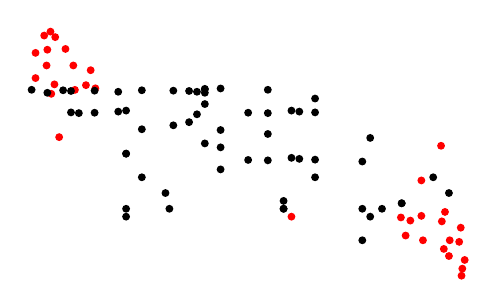
\begin{tikzpicture}
%Hotspot 1
\fill[red, thick] (-3,0) circle (0.5mm);
\fill[red, thick] (-3.2,0.2) circle (0.5mm);
\fill[red, thick] (-2.96,0.12) circle (0.5mm);
\fill[red, thick] (-2.56,0.11) circle (0.5mm);
\fill[red, thick] (-2.5,0.3) circle (0.5mm);
\fill[red, thick] (-2.7,0.05) circle (0.5mm);
\fill[red, thick] (-2.44,0.07) circle (0.5mm);
\fill[red, thick] (-2.72,0.36) circle (0.5mm);
\fill[red, thick] (-3.06,0.36) circle (0.5mm);
\fill[red, thick] (-3.05,0.56) circle (0.5mm);

\fill[red, thick] (-3.2,0.52) circle (0.5mm);
\fill[red, thick] (-2.82,0.57) circle (0.5mm);
\fill[red, thick] (-2.95,0.72) circle (0.5mm);
\fill[red, thick] (-3.09,0.74) circle (0.5mm);
\fill[red, thick] (-3.01,0.79) circle (0.5mm);

%Hotspot 2
\fill[red, thick] (2,-1.5) circle (0.5mm);
\fill[red, thick] (2.2,-1.7) circle (0.5mm);
\fill[red, thick] (1.96,-1.62) circle (0.5mm);
\fill[red, thick] (1.56,-1.61) circle (0.5mm);
\fill[red, thick] (1.5,-1.8) circle (0.5mm);
\fill[red, thick] (1.7,-1.55) circle (0.5mm);
\fill[red, thick] (1.44,-1.57) circle (0.5mm);
\fill[red, thick] (1.72,-1.86) circle (0.5mm);
\fill[red, thick] (2.06,-1.86) circle (0.5mm);
\fill[red, thick] (2.05,-2.06) circle (0.5mm);

\fill[red, thick] (2.25,-2.11) circle (0.5mm);
\fill[red, thick] (2.21,-2.31) circle (0.5mm);
\fill[red, thick] (2.18,-1.88) circle (0.5mm);
\fill[red, thick] (2.22,-2.22) circle (0.5mm);
\fill[red, thick] (1.985,-1.97) circle (0.5mm);

%Noise
\fill[red, thick] (-2.9,-0.55) circle (0.5mm);
\fill[red, thick] (1.7,-1.1) circle (0.5mm);
\fill[red, thick] (0.05,-1.56) circle (0.5mm);
\fill[red, thick] (1.95,-0.66) circle (0.5mm);

%path
\fill[black, thick] (2.05,-1.26) circle (0.5mm);
\fill[black, thick] (1.45,-1.39) circle (0.5mm);
\fill[black, thick] (-1.5,-1.46) circle (0.5mm);
\fill[black, thick] (-2.05,-1.56) circle (0.5mm);
\fill[black, thick] (-2.05,-1.46) circle (0.5mm);
\fill[black, thick] (-1.85,-1.06) circle (0.5mm);
\fill[black, thick] (-0.05,-1.46) circle (0.5mm);
\fill[black, thick] (1.45,-1.39) circle (0.5mm);
\fill[black, thick] (1.2,-1.46) circle (0.5mm);
\fill[black, thick] (1.05,-1.56) circle (0.5mm);
\fill[black, thick] (0.95,-1.46) circle (0.5mm);
\fill[black, thick] (1.85,-1.06) circle (0.5mm);
\fill[black, thick] (-0.05,-1.46) circle (0.5mm);
\fill[black, thick] (-0.85,-0.96) circle (0.5mm);
\fill[black, thick] (0.95,-0.86) circle (0.5mm);
\fill[black, thick] (0.35,-1.06) circle (0.5mm);
\fill[black, thick] (-2.05,-0.76) circle (0.5mm);
\fill[black, thick] (-1.05,-0.63) circle (0.5mm);
\fill[black, thick] (-0.85,-0.68) circle (0.5mm);
\fill[black, thick] (1.05,-0.56) circle (0.5mm);
\fill[black, thick] (-0.25,-0.51) circle (0.5mm);
\fill[black, thick] (-1.85,-0.45) circle (0.5mm);
\fill[black, thick] (-1.45,-0.4) circle (0.5mm);
\fill[black, thick] (-1.25,-0.36) circle (0.5mm);
\fill[black, thick] (-1.15,-0.26) circle (0.5mm);
\fill[black, thick] (-1.05,-0.13) circle (0.5mm);
\fill[black, thick] (-1.55,-1.26) circle (0.5mm);
\fill[black, thick] (-0.05,-1.36) circle (0.5mm);
\fill[black, thick] (-0.85,-0.46) circle (0.5mm);
\fill[black, thick] (0.95,-1.86) circle (0.5mm);
\fill[black, thick] (0.35,-0.06) circle (0.5mm);
\fill[black, thick] (-2.05,-0.76) circle (0.5mm);
\fill[black, thick] (-1.05,0.063) circle (0.5mm);
\fill[black, thick] (-0.85,0.068) circle (0.5mm);
\fill[black, thick] (-1.05,0.056) circle (0.5mm);
\fill[black, thick] (-0.25,0.051) circle (0.5mm);
\fill[black, thick] (-1.85,0.045) circle (0.5mm);
\fill[black, thick] (-1.45,0.04) circle (0.5mm);
\fill[black, thick] (-1.25,0.036) circle (0.5mm);
\fill[black, thick] (-1.15,0.026) circle (0.5mm);
\fill[black, thick] (-1.05,0.013) circle (0.5mm);

\fill[black, thick] (-3.25,0.051) circle (0.5mm);
\fill[black, thick] (-2.85,0.045) circle (0.5mm);
\fill[black, thick] (-2.45,0.04) circle (0.5mm);
\fill[black, thick] (-2.75,0.036) circle (0.5mm);
\fill[black, thick] (-2.15,0.026) circle (0.5mm);
\fill[black, thick] (-3.05,0.013) circle (0.5mm);

\fill[black, thick] (-2.65,-0.245) circle (0.5mm);
\fill[black, thick] (-2.45,-0.24) circle (0.5mm);
\fill[black, thick] (-2.75,-0.236) circle (0.5mm);
\fill[black, thick] (-2.15,-0.226) circle (0.5mm);
\fill[black, thick] (-2.05,-0.213) circle (0.5mm);

\fill[black, thick] (-0.25,-0.245) circle (0.5mm);
\fill[black, thick] (-0.5,-0.24) circle (0.5mm);
\fill[black, thick] (0.35,-0.236) circle (0.5mm);
\fill[black, thick] (0.15,-0.226) circle (0.5mm);
\fill[black, thick] (0.05,-0.213) circle (0.5mm);

\fill[black, thick] (-0.25,-0.845) circle (0.5mm);
\fill[black, thick] (-0.5,-0.84) circle (0.5mm);
\fill[black, thick] (0.35,-0.836) circle (0.5mm);
\fill[black, thick] (0.15,-0.826) circle (0.5mm);
\fill[black, thick] (0.05,-0.813) circle (0.5mm);
\end{tikzpicture}
}
\end{figure}
\end{frame}	
\begin{frame}
\frametitle{Expected Data}
	\begin{itemize}
		\item Partitional - No need for sub-clusters. %I reflektion siger vi modsat til søgning.
		\item Exclusive - Separated clusters.
		\item Partial - Need for expected outliers.
		\item Density based - Where bikes are parked for the longest time.
	\end{itemize}
	\input{slides/finding_hotspots_example_hotspot2}
\end{frame}	

\subsection{Reduction strategies}
\subsubsection{Rectangle/Ellipse}
\subsubsection{Convex Hull}
\begin{frame}
%For meget overlap.
\frametitle{Reduction strategy - Rectangle/Ellipse}
\begin{multicols}{2}
	\begin{itemize}
		\item Advantages:
		\begin{itemize}
			\item Simple
			\item Fast
		\end{itemize}
	\end{itemize}
\columnbreak
	\begin{itemize}
		\item Disadvantages:
		\begin{itemize}
			\item Very inaccurate
			\linebreak
		\end{itemize}
	\end{itemize}
\end{multicols}
\begin{figure}[h]
\fbox{
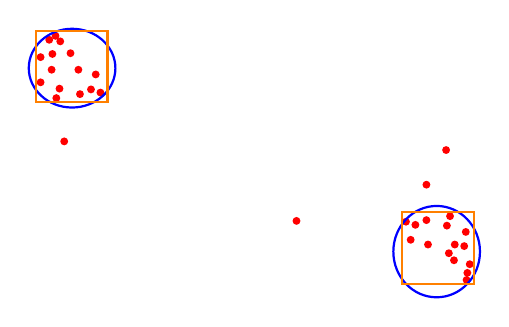
\begin{tikzpicture}
%Hotspot 1
\fill[red, thick] (-3,0) circle (0.5mm);
\fill[red, thick] (-3.2,0.2) circle (0.5mm);
\fill[red, thick] (-2.96,0.12) circle (0.5mm);
\fill[red, thick] (-2.56,0.11) circle (0.5mm);
\fill[red, thick] (-2.5,0.3) circle (0.5mm);
\fill[red, thick] (-2.7,0.05) circle (0.5mm);
\fill[red, thick] (-2.44,0.07) circle (0.5mm);
\fill[red, thick] (-2.72,0.36) circle (0.5mm);
\fill[red, thick] (-3.06,0.36) circle (0.5mm);
\fill[red, thick] (-3.05,0.56) circle (0.5mm);


\fill[red, thick] (-3.2,0.52) circle (0.5mm);
\fill[red, thick] (-2.82,0.57) circle (0.5mm);
\fill[red, thick] (-2.95,0.72) circle (0.5mm);
\fill[red, thick] (-3.09,0.74) circle (0.5mm);
\fill[red, thick] (-3.01,0.79) circle (0.5mm);

%Hotspot 2
\fill[red, thick] (2,-1.5) circle (0.5mm);
\fill[red, thick] (2.2,-1.7) circle (0.5mm);
\fill[red, thick] (1.96,-1.62) circle (0.5mm);
\fill[red, thick] (1.56,-1.61) circle (0.5mm);
\fill[red, thick] (1.5,-1.8) circle (0.5mm);
\fill[red, thick] (1.7,-1.55) circle (0.5mm);
\fill[red, thick] (1.44,-1.57) circle (0.5mm);
\fill[red, thick] (1.72,-1.86) circle (0.5mm);
\fill[red, thick] (2.06,-1.86) circle (0.5mm);
\fill[red, thick] (2.05,-2.06) circle (0.5mm);


\fill[red, thick] (2.25,-2.11) circle (0.5mm);
\fill[red, thick] (2.21,-2.31) circle (0.5mm);
\fill[red, thick] (2.18,-1.88) circle (0.5mm);
\fill[red, thick] (2.22,-2.22) circle (0.5mm);
\fill[red, thick] (1.985,-1.97) circle (0.5mm);

%Noise
\fill[red, thick] (-2.9,-0.55) circle (0.5mm);

\fill[red, thick] (1.7,-1.1) circle (0.5mm);
\fill[red, thick] (0.05,-1.56) circle (0.5mm);
\fill[red, thick] (1.95,-0.66) circle (0.5mm);

%Ellipse
%1
\draw[blue, thick] (-2.8,0.38) ellipse (5.5mm and 5mm);
%2
\draw[blue, thick] (1.83,-1.95) ellipse (5.5mm and 5.8mm);


%Rectangle
%1
\draw[orange, thick] (-3.26, 0.85) rectangle (-2.35, -0.05);
%2
\draw[orange, thick] (2.30, -2.36) rectangle (1.39 , -1.45);
\end{tikzpicture}
}
\end{figure}
\end{frame}
%\begin{frame}
%%For specifik - vores data er ikke præcis/sikker nok til at begrænse det så meget.
%\frametitle{Reduction strategy - Polygon}
%\begin{multicols}{2}
%	\begin{itemize}
%		\item Advantages:
%		\begin{itemize}
%			\item Very accurate
%			\linebreak
%		\end{itemize}
%	\end{itemize}
%\columnbreak
%	\begin{itemize}
%		\item Disadvantages:
%		\begin{itemize}
%			\item No existing algorithm
%			\item Very accurate
%		\end{itemize}
%	\end{itemize}
%\end{multicols}
%\begin{figure}[h]
\begin{tikzpicture}
%Hotspot 1
\fill[red, thick] (-3,0) circle (0.5mm);
\fill[red, thick] (-3.2,0.2) circle (0.5mm);
\fill[red, thick] (-2.96,0.12) circle (0.5mm);
\fill[red, thick] (-2.56,0.11) circle (0.5mm);
\fill[red, thick] (-2.5,0.3) circle (0.5mm);
\fill[red, thick] (-2.7,0.05) circle (0.5mm);
\fill[red, thick] (-2.44,0.07) circle (0.5mm);
\fill[red, thick] (-2.72,0.36) circle (0.5mm);
\fill[red, thick] (-3.06,0.36) circle (0.5mm);
\fill[red, thick] (-3.05,0.56) circle (0.5mm);

%Hotspot 2
\fill[red, thick] (2,-1.5) circle (0.5mm);
\fill[red, thick] (2.2,-1.7) circle (0.5mm);
\fill[red, thick] (1.96,-1.62) circle (0.5mm);
\fill[red, thick] (1.56,-1.61) circle (0.5mm);
\fill[red, thick] (1.5,-1.8) circle (0.5mm);
\fill[red, thick] (1.7,-1.55) circle (0.5mm);
\fill[red, thick] (1.44,-1.57) circle (0.5mm);
\fill[red, thick] (1.72,-1.86) circle (0.5mm);
\fill[red, thick] (2.06,-1.86) circle (0.5mm);
\fill[red, thick] (2.05,-2.06) circle (0.5mm);

%Noise
\fill[red, thick] (-2.9,-0.55) circle (0.5mm);

\fill[red, thick] (1.7,-1.1) circle (0.5mm);
\fill[red, thick] (0.05,-1.56) circle (0.5mm);
\fill[red, thick] (1.95,-0.66) circle (0.5mm);

\draw[red, thick] (-3.05,0.63) -- (-2.45,0.35);
\draw[red, thick] (-2.45,0.35) -- (-2.39,0.02);
\draw[red, thick] (-2.39,0.02) -- (-3.05,-0.05);
\draw[red, thick] (-3.05,-0.05) -- (-3.25,0.2);
\draw[red, thick] (-3.25,0.2) -- (-3.05,0.63);

\draw[red, thick] (1.39, -1.52) -- (2.05, -1.45);%(-,+) (+,-)
\draw[red, thick] (2.05, -1.45) -- (2.25, -1.7);
\draw[red, thick] (2.25, -1.7) -- (2.08, -2.13);
\draw[red, thick] (2.08, -2.13) -- (1.45, -1.8);
\draw[red, thick] (1.45, -1.8) -- (1.39, -1.52);

\end{tikzpicture}
\end{figure}
%\end{frame}
\begin{frame}
%Perfekt mellemvej mellem de to - stadig tilpas hurtig og præcis.
\frametitle{Reduction strategy - Convex Hull}
\begin{multicols}{2}
	\begin{itemize}
		\item Advantages:
		\begin{itemize}
			\item \textit{Sufficiently} accurate
			\item Multiple existing algorithms
		\end{itemize}
	\end{itemize}
\columnbreak
	\begin{itemize}
		\item Disadvantages:
	\end{itemize}
\end{multicols}
\begin{figure}[h]
\fbox{
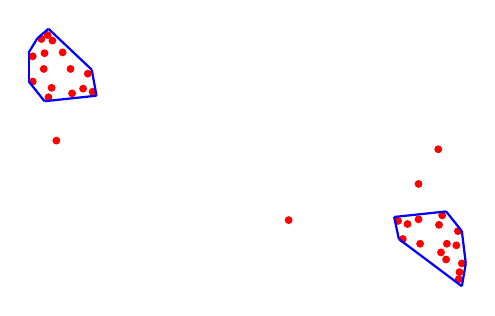
\begin{tikzpicture}
%Hotspot 1
\fill[red, thick] (-3,0) circle (0.5mm);
\fill[red, thick] (-3.2,0.2) circle (0.5mm);
\fill[red, thick] (-2.96,0.12) circle (0.5mm);
\fill[red, thick] (-2.56,0.11) circle (0.5mm);
\fill[red, thick] (-2.5,0.3) circle (0.5mm);
\fill[red, thick] (-2.7,0.05) circle (0.5mm);
\fill[red, thick] (-2.44,0.07) circle (0.5mm);
\fill[red, thick] (-2.72,0.36) circle (0.5mm);
\fill[red, thick] (-3.06,0.36) circle (0.5mm);
\fill[red, thick] (-3.05,0.56) circle (0.5mm);

\fill[red, thick] (-3.2,0.52) circle (0.5mm);
\fill[red, thick] (-2.82,0.57) circle (0.5mm);
\fill[red, thick] (-2.95,0.72) circle (0.5mm);
\fill[red, thick] (-3.09,0.74) circle (0.5mm);
\fill[red, thick] (-3.01,0.79) circle (0.5mm);


%Hotspot 2
\fill[red, thick] (2,-1.5) circle (0.5mm);
\fill[red, thick] (2.2,-1.7) circle (0.5mm);
\fill[red, thick] (1.96,-1.62) circle (0.5mm);
\fill[red, thick] (1.56,-1.61) circle (0.5mm);
\fill[red, thick] (1.5,-1.8) circle (0.5mm);
\fill[red, thick] (1.7,-1.55) circle (0.5mm);
\fill[red, thick] (1.44,-1.57) circle (0.5mm);
\fill[red, thick] (1.72,-1.86) circle (0.5mm);
\fill[red, thick] (2.06,-1.86) circle (0.5mm);
\fill[red, thick] (2.05,-2.06) circle (0.5mm);


\fill[red, thick] (2.25,-2.11) circle (0.5mm);
\fill[red, thick] (2.21,-2.31) circle (0.5mm);
\fill[red, thick] (2.18,-1.88) circle (0.5mm);
\fill[red, thick] (2.22,-2.22) circle (0.5mm);
\fill[red, thick] (1.985,-1.97) circle (0.5mm);

%Noise
\fill[red, thick] (-2.9,-0.55) circle (0.5mm);

\fill[red, thick] (1.7,-1.1) circle (0.5mm);
\fill[red, thick] (0.05,-1.56) circle (0.5mm);
\fill[red, thick] (1.95,-0.66) circle (0.5mm);



%Convex
%1
\draw[blue, thick] (-3.25,0.2) -- (-3.25,0.57);
\draw[blue, thick]  (-3.25,0.57) -- (-3.14, 0.75);
\draw[blue, thick]  (-3.14, 0.75) -- (-3.0, 0.87);
\draw[blue, thick]  (-3.0, 0.87) -- (-2.45,0.35);
\draw[blue, thick] (-2.45,0.35) -- (-2.39,0.02);
\draw[blue, thick] (-2.39,0.02) -- (-3.05,-0.05);
\draw[blue, thick] (-3.05,-0.05) -- (-3.25,0.2);


%2
\draw[blue, thick] (1.39, -1.52) -- (2.05, -1.45);%(-,+) (+,-)
\draw[blue, thick] (2.05, -1.45) -- (2.25, -1.7);
\draw[blue, thick] (2.25, -1.7)  -- (2.3, -2.11);
\draw[blue, thick] (2.3, -2.11)  -- (2.25, -2.4);
\draw[blue, thick] (2.25, -2.4)  -- (1.45, -1.8);
%\draw[blue, thick] (2.25, -1.7) -- (2.08, -2.13);
%\draw[blue, thick] (2.08, -2.13) -- (1.45, -1.8);
\draw[blue, thick] (1.45, -1.8) -- (1.39, -1.52);

\end{tikzpicture}
}
\end{figure}
\end{frame}
\section{Predicting Behaviour}
\begin{frame}{The prediction problem}
\begin{center}
How much time will it take before a bike will be \emph{in a given hotspot}

\includegraphics[width=0.8\linewidth]{graphics/biketime}
\end{center}

\end{frame}

\subsection{Modeling the system}

\begin{frame}{Simple hotspot model}
\begin{figure}[h]
\begin{tikzpicture}[->,>=stealth',shorten >=1pt,auto,node distance=10cm,
  thick,main node/.style={circle,fill=blue!20,draw,font=\sffamily\Large\bfseries}]

  \node[main node] (1) {$h_1$};
  \node[main node] (2) [right of=1] {$h_2$};

  \path[every node/.style={font=\sffamily\small}]
    (1) edge [bend left] node {0.3} (2)
        edge [loop left] node {0.7} (1)
    (2) edge [bend left] node {0.6} (1)
        edge [loop right] node {0.4} (2);
\end{tikzpicture}
\caption{A Markov chain model with two hotspots}
\label{markov:model:simple}
\end{figure}
\end{frame}

\begin{frame}
\begin{center}
Where do we place the black bike?	
\includegraphics[scale=0.7]{graphics/world}
\end{center}
\end{frame}

\begin{frame}{Departure state model}
\begin{figure}
\begin{tikzpicture}[->,>=stealth',shorten >=1pt,auto,node distance=4cm,
  thick,main node/.style={circle,fill=blue!20,draw,font=\sffamily\Large\bfseries}]

  \node[main node] (B1) {$B_1$};
  \node[main node,font=\sffamily\small] (D1) [right = 2cm of B1] {$D_1$};
  \node[main node,font=\sffamily\small] (D2) [right of=D1] {$D_2$};
  \node[main node] (B2) [right = 2cm of D2] {$B_2$};

  \path[every node/.style={font=\sffamily\small}]
    (B1) edge [bend left] node {0.05} (B2)
         edge [loop left] node {0.65} (B1)
         edge [bend left] node[below] {0.3} (D1)
    (B2) edge [bend left] node {0.15} (B1)
         edge [loop right] node {0.35} (B2)
         edge [bend left] node[above] {0.5} (D2)
    (D1) edge [bend left] node[above] {0.1} (B1)
         edge [loop right] node {0.6} (D1)
         edge [bend left] node[below left] {0.3} (B2)
    (D2) edge [bend left] node[below] {0.1} (B2)
         edge [loop left] node {0.7} (D2)
         edge [bend left] node[above right] {0.2} (B1);
\end{tikzpicture}
\caption{A Markov chain model of two bike stations with departure states}
\label{markov:model:complex}
\end{figure}
\end{frame}

\subsection{Creating the model}

\begin{frame}{}
	
\begin{center}
We want to generate the model with data from the GPS receivers on the bikes
	
\includegraphics[width=0.8\linewidth]{graphics/build_the_model}
\end{center}

\end{frame}

\begin{frame}{The algorithm}
\def\HiLi{\leavevmode\rlap{\hbox to \hsize{\color{yellow!50}\leaders\hrule height .8\baselineskip depth .5ex\hfill}}}


\scalebox{0.8}{
	
\begin{algorithm}[H]
\SetAlgoNoEnd
\textbf{CreateModel}($H, G, step$)\\
Let $M$ be an empty $n \times n$ matrix with $n = 2|H|$ \\
\ForEach{$b \in B$}
	{
	$g \leftarrow G(b).first$\\
\HiLi	$L(b) \leftarrow \textbf{NearestState}(H, g)$
	}
 Let $d \leftarrow G.first.date$\\
Let $l \leftarrow G.last.date$\\
\While{$d \leq l$}
	{
	\ForEach{$b \in B$}
		{
		$g \leftarrow G(b, d)$\\
		$n \leftarrow \textbf{NearestState}(H, g)$\\
		\If{$n \in D \wedge L(b) \in D$}
			{
		$n \leftarrow L(b)$
			}
		\ElseIf{$n \in D \wedge L(b) \in H$}
			{
			$n \leftarrow L(b).departure$
			}
		}
	$d \leftarrow \text{Add}(d, step)$
	}
Normalize $M$\\
\Return{M}
\end{algorithm}

}
\end{frame}

\subsection{Predicting with the model}

\begin{frame}{}
	
\begin{center}
The initial distribution of bikes in the system

\includegraphics[scale=0.7]{graphics/initialworld}
	
$ (8,2,6,0) $
\end{center}
\end{frame}

\begin{frame}
	
\begin{center}	
	
$ P_i \times \tau_M = P_{i+1}$\\
		
		
$$
(8, 2, 6, 0)
\begin{bmatrix}
0.65 & 0.3 & 0.05 & 0\\
0.1  & 0.6 & 0.3  & 0\\
0.15 & 0   & 0.35 & 0.5\\
0.2  & 0   & 0.1  & 0.7
\end{bmatrix}
=
(6.3, 3.6, 3.1, 3)
$$
\end{center}
\end{frame}

\begin{frame}{Predicting with accumulation}
Simulating that bikes never leave the hotspot where the user is waiting

$$ \begin{bmatrix}
	{\color{red}1} & {\color{blue}0} & \color{blue} 0& {\color{blue}0}\\
	0.1  & 0.6 & 0.3  & 0\\
	0.15 & 0   & 0.35 & 0.5\\
	0.2  & 0   & 0.1  & 0.7
\end{bmatrix}
 $$
\end{frame}


\begin{frame}
$$
(8, 2, 6, 0)
\begin{bmatrix}
1 & 0 & 0 & 0\\
0.1  & 0.6 & 0.3  & 0\\
0.15 & 0   & 0.35 & 0.5\\
0.2  & 0   & 0.1  & 0.7
\end{bmatrix}
=
(9.1,1.2,2.7,3)
$$
	
$$
(9.1,1.2,2.7,3)
\begin{bmatrix}
1 & 0 & 0 & 0\\
0.1  & 0.6 & 0.3  & 0\\
0.15 & 0   & 0.35 & 0.5\\
0.2  & 0   & 0.1  & 0.7
\end{bmatrix}
=
(10.225,0.72,1.605,2.37)
$$
	
\end{frame}
\section{Demo}
\subsection{Simulation}

\begin{frame}
\frametitle{Configuration}
\begin{itemize}
\item A system where locations are retrieved from GPS receivers.
\item There is no such system yet.
\item Simulate such a system:
\begin{itemize}
\item $\pm$30 seconds delay from the GPS receiver.
\item The GPS Data is perturbed.
\item Lost GPS Data is not taken into account.
\end{itemize}
\end{itemize}
\end{frame}

\begin{frame}
\frametitle{Setup}
\begin{itemize}
\item 5 bikes.
\item 3 addresses.
\item The BikeVisualizer shows us the GPS data and how they are interpreted.
\end{itemize}
\end{frame}



\section{Future Work}
\subsection{Conclusion}
\begin{frame}{There will be no conclusion}
I don't plan on including a slide for the conclusion.
I don't think I can say anything interesting about the text in the conclusion.
\end{frame}

\end{document}